\paragraph{QuizziPedia::Back-End::App::Routers::QuizRouter}
\label{QuizziPedia::Back-End::App::Routers::QuizRouter}
\begin{figure}[ht]
	\centering
	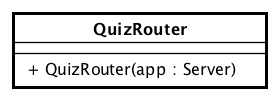
\includegraphics[scale=0.45]{UML/Classi/Back-End/QuizziPedia_Back-End_App_Routers_quizRouter.png}
	\caption{QuizziPedia::Back-End::App::Routers::QuizRouter}
\end{figure}
\FloatBarrier
	\begin{itemize}
		\item \textbf{Descrizione} 
		Classe che gestisce le richieste relative alle operazioni riguardanti un questionario. Componente ConcreteHandler del design pattern Chain of responsibility.
		\item \textbf{Utilizzo} 
		Viene utilizzata per chiamare il controller che si occupa di gestire le API relative ad un questionario.
		\item \textbf{Relazioni con altre classi} 
		\begin{itemize}
		\item \textbf{IN \texttt{Server}} \\
			Classe che avvia il server. Nello specifico apre una connessione al database tramite Mongoose, invoca il middleware Express passando un riferimento al database MongoDB come parametro in modo che possa configurarsi con esso, invoca il middleware Passport ed infine si mette in ascolto su una determinata porta. È il componente client del design pattern Chain of responsibility. Utilizza i moduli Mongoose, Express, Passport;
		\item \textbf{OUT \texttt{ErrorHandler}} \\
			Classe middleware per la gestione degli errori. Ritorna al client un oggetto di tipo Response con stato HTTP 500 e descrizione dell'errore in formato JSON. È un componente ConcreteHandler del design pattern Chain of responsibility;
		\item \textbf{OUT \texttt{NotFoundHandler}} \\
			Classe che si occupa della gestione dell'errore di pagina non trovata. Componente ConcreteHandler del design pattern Chain of responsibility;
		\item \textbf{OUT \texttt{QuizController}} \\
			Classe che raggruppa i vari controllers responsabili delle operazioni riguardanti un questionario attraverso require.
		\end{itemize}
		\item \textbf{Metodi} 
		\begin{itemize}
		\item \texttt{+ QuizRouter(app: Server)} \\
		Contiene diverse route che vengono configurate all’avvio del server. Quest’ultime ricevono le richieste del client e passano il controllo al ConcreteHandler successivo. \\
		\textbf{Parametri}:
		\begin{itemize}
		\item \texttt{app : Server} \\
		Rappresenta l’istanza del server su cui configurare i route che mappano i controllers specifici.
		\end{itemize}
		\end{itemize}
	\end{itemize}